\section{Example: Wheel Brake System}

%\mike{Move the generic description to a section right after the ``safety'' section along with the ARP figure.  Leave the modeling that we did in AADL here.  That way we can reference it in the MBSA sections.}
%\danielle{The whole nominal model description is here. The modeling we did is in the faults section.}

As a preliminary case study, we utilized the Wheel Brake System (WBS) described in \cite{AIR6110} (previously found in ARP4761 Appendix L). This ficticious aircraft system was developed to illustrate the design and safety analysis principles of ARP4754A and ARP4761.  The WBS is installed on the two main aircraft landing gears and is used during taxi, landing, and rejected take off. Braking is either commanded manually using brake pedals or automatically by a digital control system with no need for the pedals (autobrake). When the wheels have traction, the autobrake function will provide a constant smooth deceleration.

\begin{figure}
\begin{center}
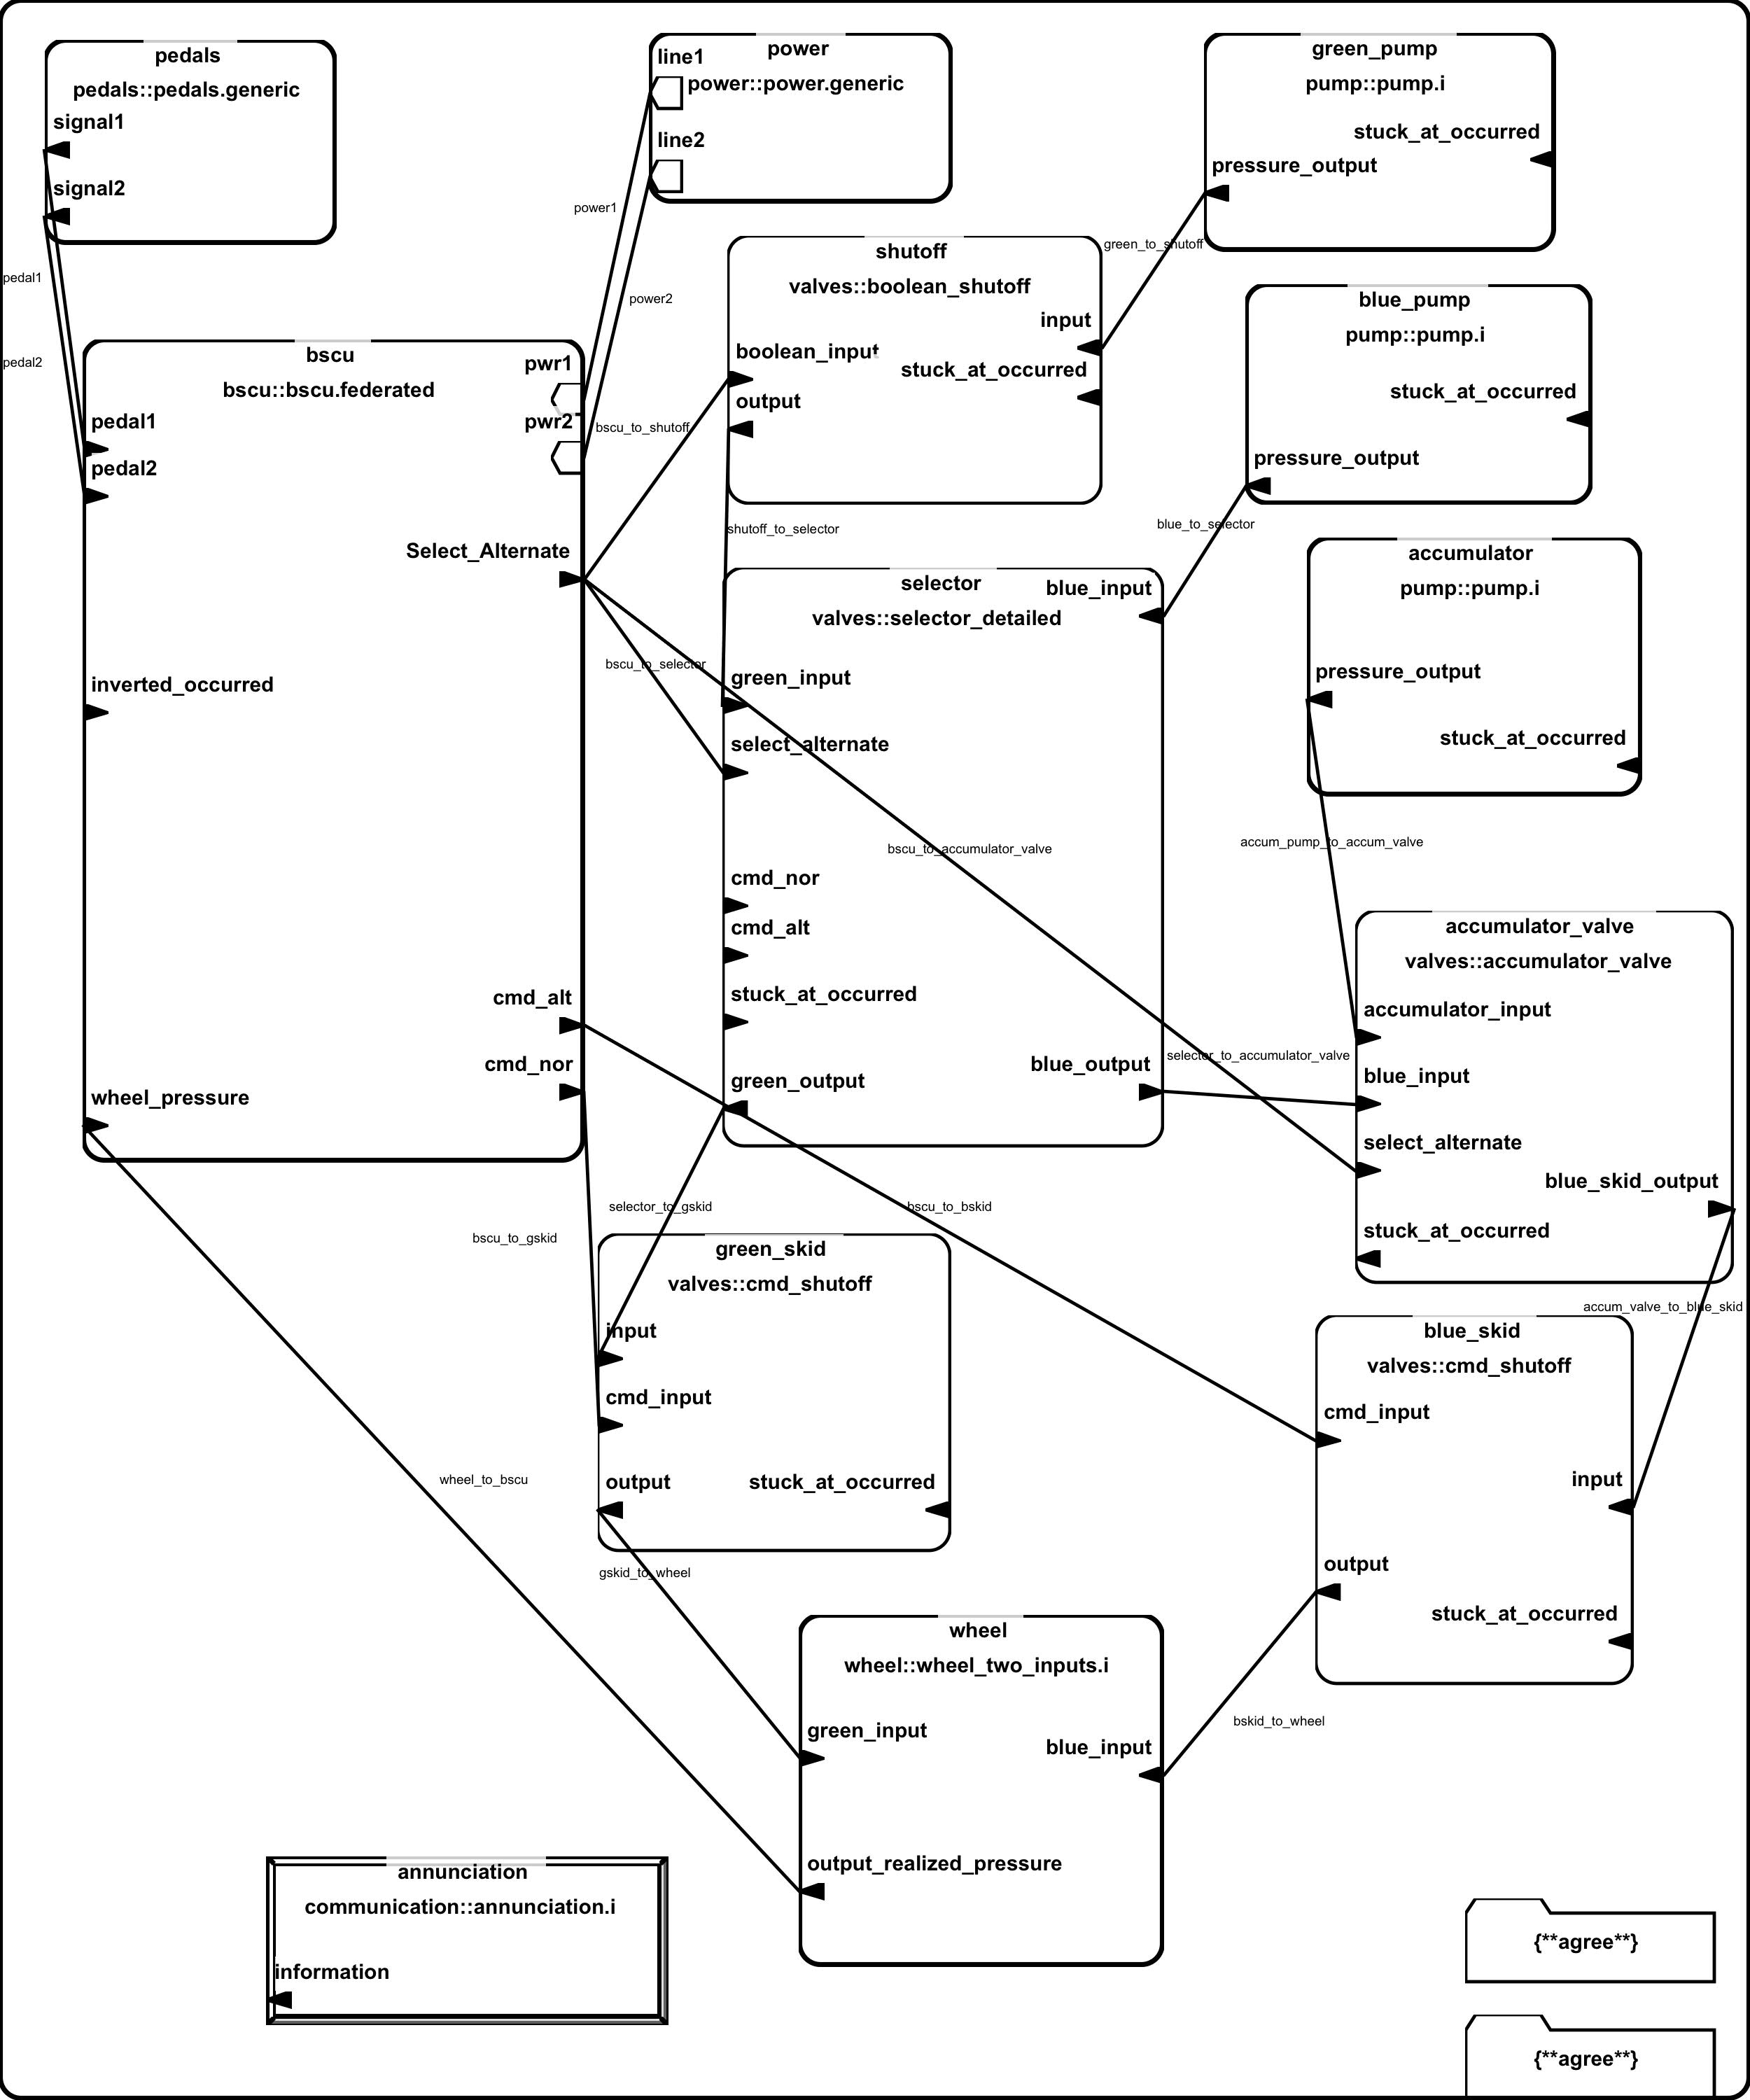
\includegraphics[width=\textwidth]{images/wbsfederated3.jpg}
\caption{AADL Simple Model of the Wheel Brake System }
\label{fig:wbs_ima}
\end{center}
\end{figure}

Each wheel has a brake assembly that can be operated by two independent hydraulic systems (designated green and blue). In normal braking mode, the green hydraulic system operates the brake assembly.  If there is a failure in the green hydraulics, the system switches to alternate mode which uses the blue hydraulic system.  The blue system is also supplied by an accumulator which is a device that stores hydraulic pressure that can be released if both of the primary hydraulic pumps (blue and green) fail. The accumulator supplies hydraulic pressure in Emergency braking mode.

Switching between the hydraulic pistons and pressure sources can be commanded automatically or manually. If the hydraulic pressure in the green supply is below a certain threshold, there is an automatic switchover to the blue hydraulic supply. If the blue hydraulic pump fails, then the accumulator is used to supply hydraulic pressure.

In both normal and alternate modes, an anti-skid capability is available. In the normal mode, the brake pedal position is electronically fed to a computer called the Braking System Control Unit (BSCU). The BSCU monitors signals that denote critical aircraft and system states to provide correct braking function, detect anomalies, broadcast warnings, and sent maintenance information to other systems.

\subsection{Nominal System Model}
\label{sec:nominal}
The WBS AADL model of the nominal system behavior consists of mechanical and digital components and their interconnections, as shown in Figure~\ref{fig:wbs_ima}. The following section describes this nominal model from which the fault model was generated.

\paragraph{Wheel Braking System (WBS)}
The highest level model component is the WBS. It consists of the BSCU, green and blue hydraulic pressure lines (supplied by the green pump  and blue pump/accumulator respectively), a Selector which selects between normal and alternate modes of hydraulic pressure, and the wheel system. The WBS takes inputs from the environment including PedalPos1, AutoBrake, DecRate, AC\_Speed, and Skid. All of these inputs are forwarded to the BSCU to compute the brake commands.

\paragraph{Braking System Control Unit (BSCU)}
The BSCU is the digital component in the system that receives inputs from the WBS. It also receives feedback from the green and blue hydraulic lines and two power inputs from two separate power sources. The BSCU is composed of two command and monitor subsystems each powered independently from separate power sources. The pedal position is provided to these units and when skidding occurs, the command and monitor units will decrease the pressure to the brakes.
The command unit regulates the pressure to the brakes in the green hydraulic line through the command cmd\_nor. Computing this command requires both the brake requested power and the skid information. The command unit also regulates the pressure in the blue hydraulic line in order to prevent skidding which it does through the cmd\_alt command. The monitor unit checks the validity of the command unit output.

The BSCU switches from normal to alternate mode (blue hydraulic system) when the output from either one of its command units is not valid or the green hydraulic pump is below its pressure threshold.  Once the system has switched into alternate mode, it will not switch back into normal mode again.

\paragraph{Hydraulic Pumps}
There are three hydraulic pumps in the system, green pump (normal mode), blue pump (alternate mode), and accumulator pump (emergency mode). Each pump provides pressure to the system and is modeled in AADL as a floating point value.

\paragraph{Shutoff Valve}

The shutoff valve is situated between the green pump and the selector. It receives an input from the BSCU regarding valve position and regulates the pressure coming through the green pipe accordingly.

\paragraph{Selector Valve}
The selector receives inputs from the pumps regarding pressure output and the BSCU regarding which mode the system is in. It will output the appropriate pressure from green, blue, or accumulator pump. An added requirement of the selector system is that it will only output pressure from one of these sources. Thus, the case of having pressure supplied to the wheels from more than one pump is avoided. The Selector takes the two pipe pressures (green and blue) as input, selects the system with adequate pressure and blocks the system with inadequate pressure. If both systems have pressure greater than the threshold, the AADL selects normal mode as the default.

\paragraph{Skid Valves}
The blue\_skid and green\_skid valves receive input from the selector as pressure coming through the respective pipes as well as input from the BSCU that commands normal or alternate mode. The skid valves will use these inputs to choose between the green or the blue pressure to send to the wheel.

\subsection{Modeling Nominal System Behavior}
In order to reason about behaviors of complex system architectures, we have developed a compositional verification tool for AADL models.
Our tool, the {\em Assume-Guarantee Reasoning Environment} (AGREE) \cite{NFM2012:CoGaMiWhLaLu}  is based on {\em assume-guarantee} contracts that can be added to AADL components.  The language used for contract specification is based on the LUSTRE dataflow language~\cite{Halbwachs91:IEEE}. The tool allows scaling of formal verification to large systems by splitting the analysis of a complex system architecture into a collection of verification tasks that correspond to the structure of the architecture.

We use AGREE to specify behavioral contracts corresponding to the behaviors expected of each of the WBS components. An example of a contract is shown in Figure~\ref{fig:agreeContract}.
%

\begin{figure}
\begin{center}
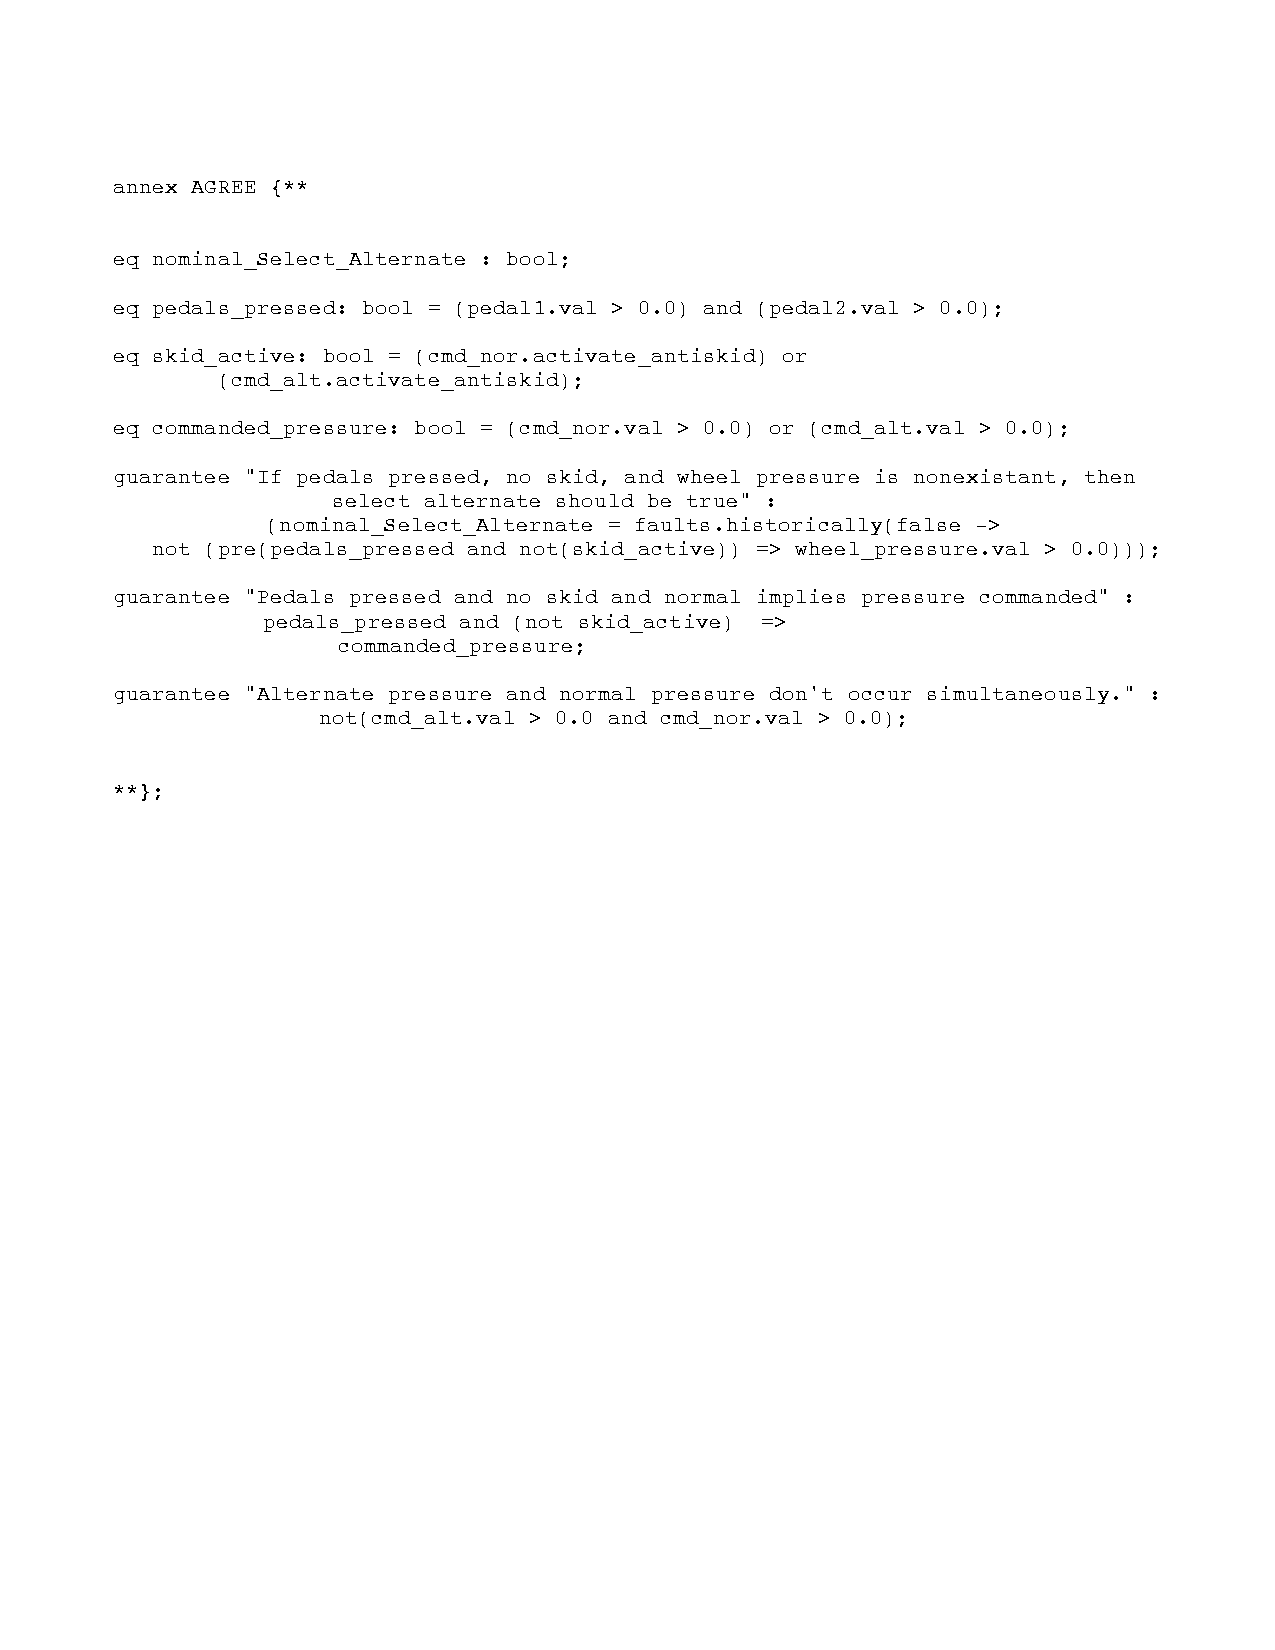
\includegraphics[trim=60 480 50 60,clip,width=\textwidth]{images/bscu.pdf}
\caption{AGREE Contract for BSCU }
\label{fig:agreeContract}
\end{center}
\end{figure}

\iffalse

\subsection{Nominal System Modeling}
\mike{KEEP HERE!}
A formal specification of the nominal system model consists of mechanical and digital components and their interconnections.

The highest level component is the Wheel Braking System (WBS). It consists of a digital control unit, the BSCU, and normal and alternate hydraulic pressure lines (supplied by green pump and blue pump/accumulator respectively). The system takes inputs from the environment including PedalPos1, AutoBrake, DecRate, AC\_Speed, and Skid. All of these inputs are forwarded to the BSCU to compute the brake commands. The outputs of the WBS are normal\_pressure, alternate\_pressure, and System\_Mode (normal, alternate, EMERGENCY).

\subsection{Braking System Control Unit (BSCU)}
The BSCU is the digital component in the system that receives inputs from the WBS. It also receives feedback from the normal and alternate lines and two power inputs from two separate power sources.

\fi

